\documentclass[a4paper]{article}

\usepackage{graphicx}

\title{MTF Mapper}
\author{F. van den Bergh (fvdbergh@gmail.com)}

\begin{document}
\maketitle

\section{Overview}
The MTF mapper package offers a collection of tools to measure Modulation
Transfer Function (MTF) values in images. It does this by computing the edge
spread function of a step edge in an image. (details of paper).

MTF mapper offers fully automated operation, producing the following
outputs:
\begin{enumerate}
    \item Annotated images, where the MTF50 value of an edge is drawn on top
of the edge itself;
    \item Profile data sets, where the MTF50 values are represented in a
one-dimensional projection of the image. This is the tool you want if you
are interested in objectively adjusing your DSLR autofocus fine-tuning.
    \item MTF surface images, where you can visualise the MTF50 values
across the focal plane, to see the image centre MTF50 relative to edge MTF50,
for example.
\end{enumerate}

MTF mapper expects images containing dark rectangular objects on light
backgrounds; the objects can be slightly out-of-square, e.g., trapezoids or
parallelograms, provided the interior angles are at least reasonably close
to 90$^\circ$.

Special test charts are required for Profile mode.

Special test charts are also required for MTF surface mode.

\section{Modes}
\subsection{Annotation}
No explanation required, really. Input images are searched for rectangular
objects. Once found, the MTF50 value will be computed across each edge of
all the rectangular objects. The resulting value is drawn on top of each
edge, and the result saved as \textrm{annotated.png} by default.

\subsection{Profile}
Using a special test chart that looks like
Figure~\ref{fig:profile_test_chart}, the program will construct a profile
such as the one shown in Figure~\ref{fig:sample_profile}. The test chart
contains a reference block --- the large one in the centre of the chart. The
following steps can be used to callibrate the autofocus fine-tuning of a
DSLR:

\begin{figure}
\centering
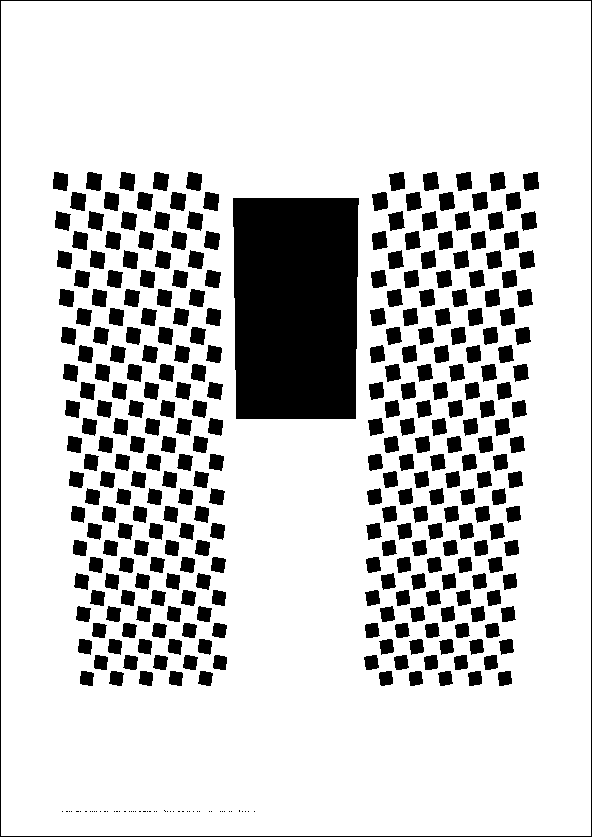
\includegraphics[width=0.4\textwidth]{figures/mtf_profile_test_chart}
\caption{Example of Profile mode test chart}
\label{fig:profile_test_chart}
\end{figure}

\begin{figure}
\centering
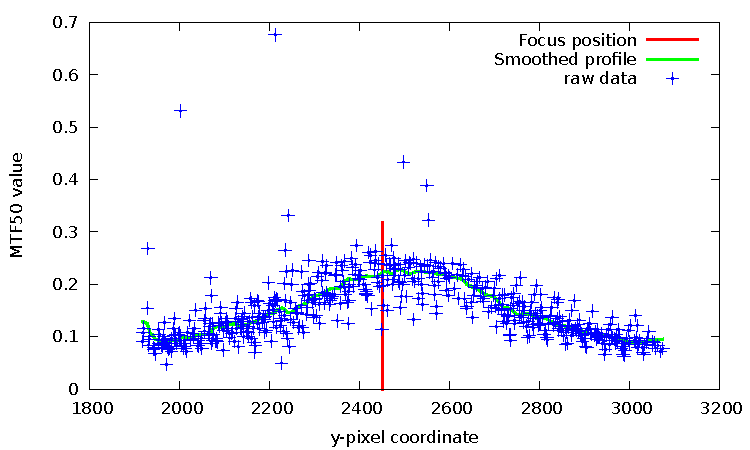
\includegraphics[width=0.95\textwidth]{figures/sample_profile}
\caption{Example of Profile profile generated by MTF mapper}
\label{fig:sample_profile}
\end{figure}

\begin{enumerate}
    \item Print out the test chart at a large enough scale. Ideally, your
test chart must be large enough so that you can use it at a distance of
$30\times$ the focal length of your lens. Position your camera so that you
see the chart from an angle of at least $45^\circ$ --- the idea is that you
want some of the small blocks to be in front of the plane of focus, and some
of the blocks behind the plane of focus. The reference edge should be
exactly at the plane of focus, but since you are reading this, I take it you
are still trying to adjust the autofocus fine-tuning to achieve this.
    \item Using a tripod (and remote release / timed release), take a
picture of the test chart \emph{with your chosen (centre recommended)
autofocus sensor stradling the edge of the reference block}. (TODO: add more
pictures to illustrate)
    \item Feed the captured image through MTF mapper to produce a profile
(such as illustrated in Figure~\ref{fig:sample_profile}. The vertical red
line denotes the position of the autofocus reference edge (at least, the one
you should have been using to focus \ldots). The green curve (or blue
points) records the MTF50 values measured along the $y$-axis of the image.
Since the test chart was at a $45^\circ$ angle with respect to the lens
axis, the $y$-axis of the image is a measure of the distance from the
camera. MTF50 values measured at different $y$-values thus indicate the
sharpness, or degree of focus, at that specific distance from the camera.
The peak of the green curve represents the plane of focus --- the objective
is to line up the peak of the green curve with the red vertical line.
    \item This procedure should now be repeated at various autofocus
fine-tuning settings on your camera. You should be able to see the peak of
the green curve shift left or right as you adjust this value. I recommend
capturing your images in batches, first stepping your autofocus fine-tuning
through the range in large steps, running the images through MTF mapper, and
then repeating this in the optimal range with smaller steps until you are
satisfied that you have calibrated your autofocus fine-tuning to the desired
level of accuracy.
\end{enumerate}

TODO: diagrams of the set-up, more detail.


\subsection{MTF surface}
Using any test chart with a regular grid of rectangles (as illustrated in
Figure~\ref{fig:surface_test_chart}, you can measure the acuity of your
lens/camera system as it varies across the focal plane. Just shoot the chart
at a reasonable distance, making sure that it covers the entire viewfinder.

TODO: more detail.

\begin{figure}
\centering
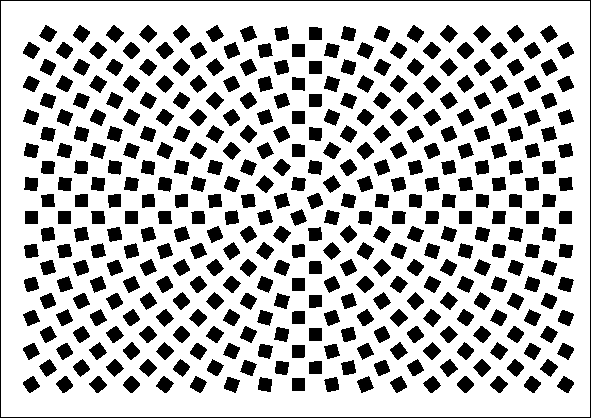
\includegraphics[width=0.5\textwidth,angle=90]{figures/mtf_surface_test_chart.pdf}
\caption{Example of an MTF surface mode test chart}
\label{fig:surface_test_chart}
\end{figure}


\end{document}
